%% 内容梗概

%% プリアンブル %%%%%%%%%%%%%%%%%%%%%%%%%%%%%%%%%%%%%%%%%%%%%%%%%%%%%%%%
\documentclass[a4j]{jarticle}

\usepackage{kut-abstract}
%\usepackage[dvips]{graphicx}
\usepackage[dvipdfmx]{graphicx}
\usepackage{utf}
%% 表題 %%%%%%%%%%%%%%%%%%%%%%%%%%%%%%%%%%%%%%%%%%%%%%%%%%%%%%%%%%%%%%%%
%% 注意! 情報学群生の場合は,以下の \ScInfo を有効にすること.
%\ScInfo %% 情報学群生の場合

\Bachelor	%% 卒業研究論文梗概の場合
%\Project	%% プロジェクト研究報告書梗概の場合
%\Seminar	%% 特別研究セミナー課題研究報告書梗概の場合
%\Master	%% 修士学位論文(情報システム工学コース)梗概の場合
%\Doctorate	%% 博士学位論文(情報システム工学コース)梗概の場合
%\English	%% 英語の場合

\Eyears{2017}
\Etitle{English Title}
%\idnumber{}
\Eauthor{YAMASAKI, Naoyuki}
\Eaffiliate{Iwata Lab.}

%% 本文 %%%%%%%%%%%%%%%%%%%%%%%%%%%%%%%%%%%%%%%%%%%%%%%%%%%%%%%%%%%%%%%%

\years{平成29}
\title{LSTM-RNN用アクセラレータ回路の負荷割当法の検討}
\idnumber{1180386}
\author{山 \UTF{FA11} ~~尚 之}
\affiliate{コンピュータ構成学研究室}

%% 本文 %%%%%%%%%%%%%%%%%%%%%%%%%%%%%%%%%%%%%%%%%%%%%%%%%%%%%%%%%%%%%%%%
\begin{document}
\begin{Abstract}

 \section{はじめに}

言語処理,音声認識の分野で長期短期記憶LSTM(Long Short-term Memory)が注目されており,
組込みシステムでリアルタイム翻訳などに用いる場合アクセラレータ回路を使用し,
高速に処理する必要がある.
LSTM-RNN(Recurrent Neural Network)は
一般的な人工ニューラルネットワークANN(Artificial Neural Network)に比べ,
3種のゲートと自状態の重みが必要で演算量が大きくなる.
そのため,LSTM-RNN用アクセラレータの要求が求められるようになっている.

先行研究として,LSTMを含む微分可能ニューラルコンピュータDNC(Differentiable Neural Computer)
用単一コアの提案がされている\cite{bib:pre-method}.
しかし,シングルコアでは処理性能に限界があるためマルチコア化が求められる.

本研究では,LSTMをマルチコアで動作させる場合の負荷割り当てについて最適な方法の検討を行う.



 \section{負荷割り当て方法}
 負荷割り当ての方法は図1のフロー図に示す3方向の軸に沿った方法が考えられる.
 \begin{figure}[h]
  \centering
  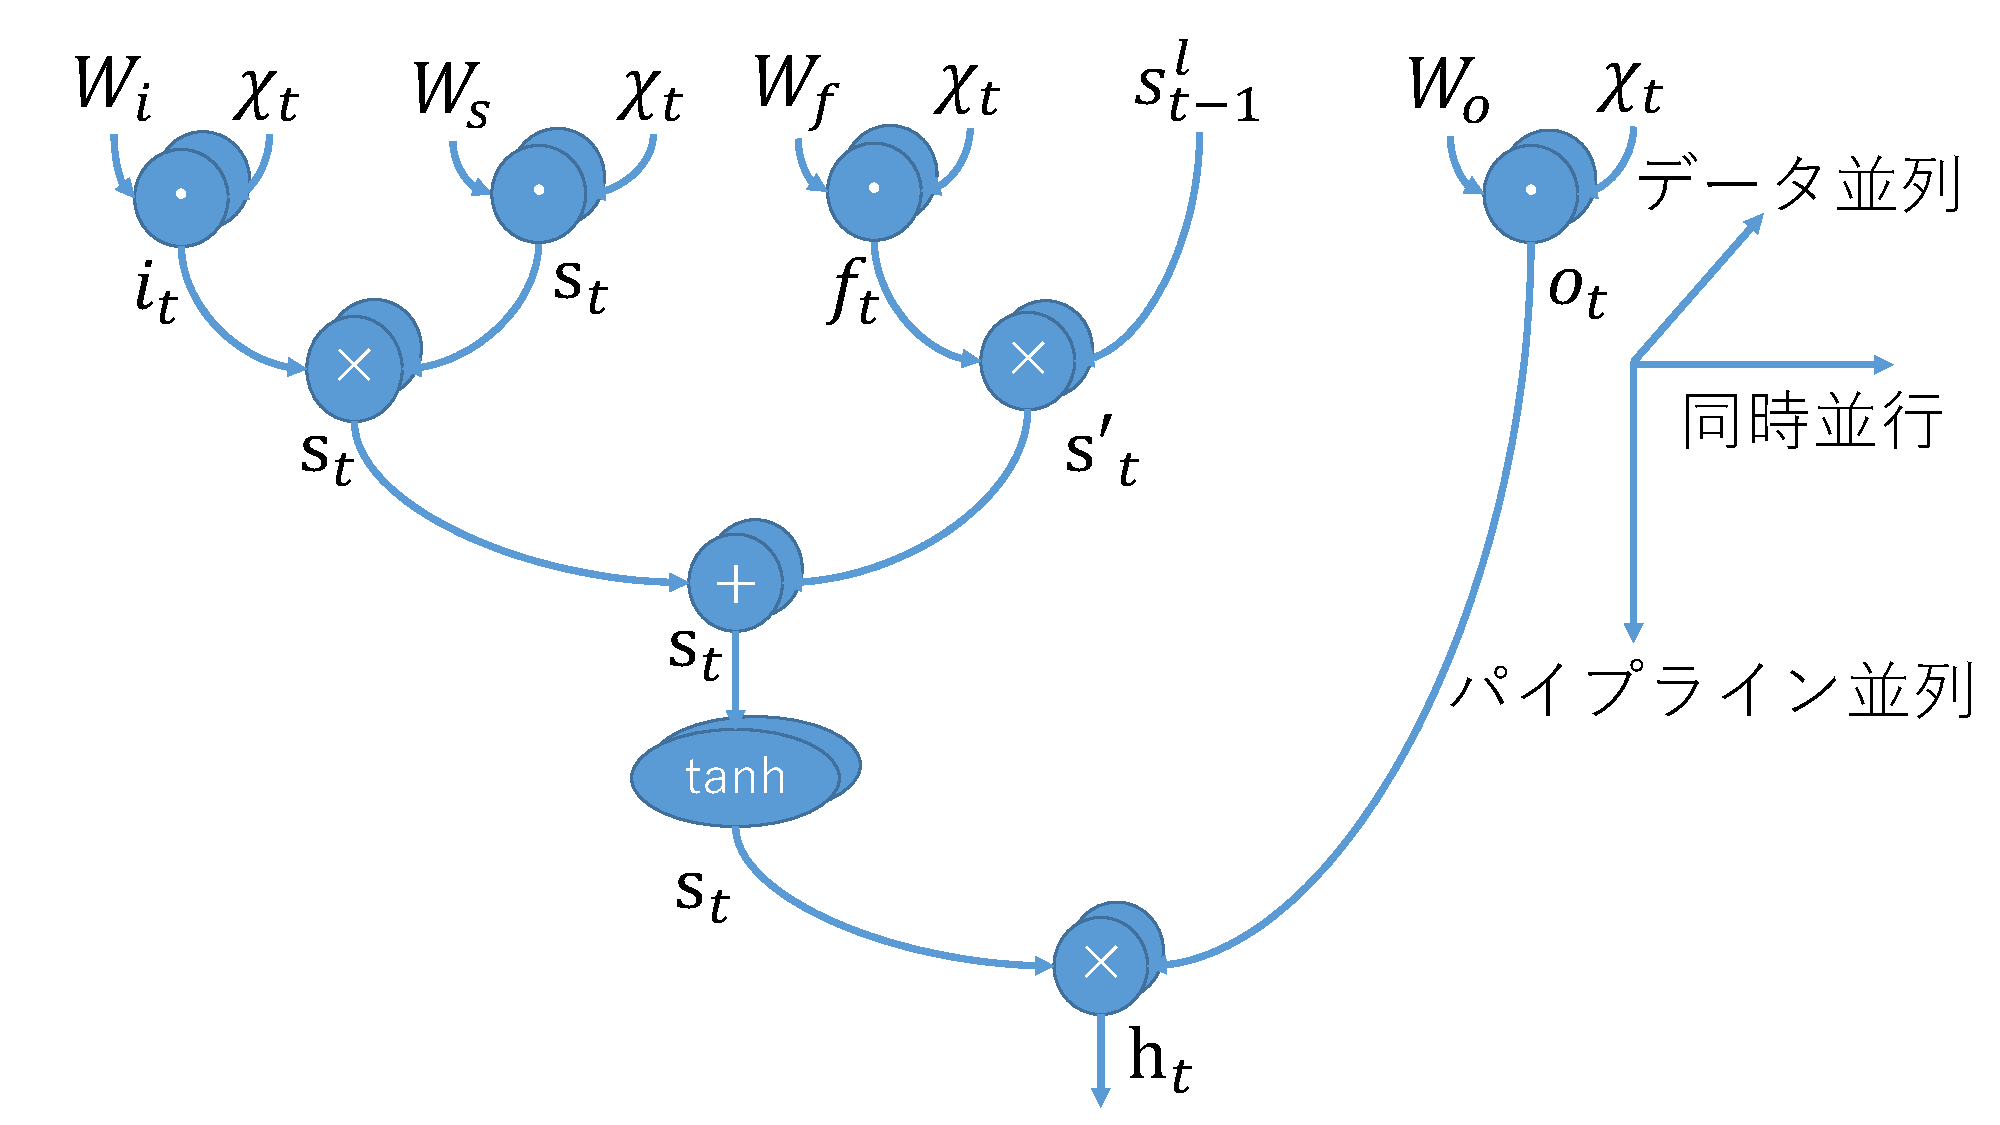
\includegraphics[scale=0.25]{flow.eps}
  \caption{LSTMの計算フロー図}
 \end{figure}


同時実行並列方向とパイプライン並列方向の負荷割り当ては,
図1の演算命令を左右と上下にそれぞれ分け,
各コアに割り振られた命令を実行する方法である.
データ並列方向の負荷割り当ては全命令を各コアで実行するが,
各演算に必要な行列やベクトルの要素を半分に分ける方法である.
データ並列方向の負荷割当ではデータの重複を限りなく少なくできるが,
演算に必要なデータを半分にして演算を行うため,
図1にはない足し合わせの処理が必要となる.


 \section{性能の見積もり}
 この3つの負荷割り当て方法をコア数50,中間層のニューロン数200,入力数を50とし,
 1回の演算処理にかかる時間,1回の通信にかかる時間,
 1要素のデータを保存するためのメモリ領域をそれぞれ1とし,
 実行時間と回路面積を算出し比較を行った結果を表1に示す.
 実行時間は演算時間と通信時間を足し合わせた値である.
 また,性能の指標として実行時間と面積の積をとる.
 この値が低い値であるほど1コアあたりの負荷が低く性能が高いと言える.

 結果として,データ並列方向に負荷割り当てを行った場合,
 二番目に性能の良い同時実行並列方向の割り当てに比べ,
 18\%低負荷での実行が可能であるという見積もり結果が得られた.

 また,通信方法として,Bus,Interconnection Network,
 Crossbarの3種類が主な手法として考えられが,
 どの方法を選択したとしても,
 同程度負荷を軽減させることが可能であるという結果が得られた.

 \begin{table}[htb]
    \begin{center}
      \caption{各負荷割り当て方法の負荷見積もり}
      \begin{tabular}{|c||c|c|c|}\hline
       負荷割り当て方法 & 実行時間 & 回路面積 & 性能 \\ \hline
       同時実行並列 & 202250 & 5150 & 1.24*10$^{10}$ \\ \hline
       パイプライン並列 & 301650 & 5150 & 1.81*10$^{10}$ \\ \hline
       データ並列 & 203050 &  4169 & 8.92*10$^{9}$ \\ \hline
     \end{tabular}
   \end{center}
 \end{table}


次に,最も性能の高い結果が得られた,
データ並列方向の負荷割り当てについて稼働率(実行命令数/(実行命令数+NOP命令実行数))を求める.
マルチコアで動作させる場合,通信回路が他のコアとの通信に使われていて,通信が行えない時などに,
処理を行わないNOP命令が実行される.
このNOP命令が行われているとき,演算処理は進まないためそのコアは止まった状態となり稼働率が低下する.
LSTMを実行した場合,
1タイムステップで1コアあたり実行されるNOP命令は〇〇回であり,稼働率は△△\%であった.

 \section{まとめ}
負荷の割り当て方法として,
データ並列方向の負荷割り当てが3つの割り当て方法の中で,
実行時間,回路面積の観点から最も性能が高くなるという見積もり結果が得られた.
今後,この見積もりをもとに実装を行い,実際の性能評価を行う.


%% 参考文献 %%%%%%%%%%%%%%%%%%%%%%%%%%%%%%%%%%%%%%%%%%%%%%%%%%%%%%%%%%%%
\begin{thebibliography}{99}
 \bibitem{bib:pre-method} Akane Saito, Yuki Umezaki, and Makoto Iwata,
  ``Hardware Accelerator for Differentiable Neural Computer and Its FPGA Implementation,
  ''PDPTA'17, pp.232-238, July 2017.
\end{thebibliography}

\end{Abstract}
\end{document}
